\section{Randomized per-hypothesis depth and optimal mixing}
\label{sec:randomized-programming}

The previous algorithms return one tree. For a fixed prior, expected
depth averages that tree's depths over hypotheses; deterministic
maximum depth protects the slowest hypothesis in that same tree.
We now consider a separate extension: preprocessing returns a small
collection of legal trees and probabilities for choosing among them.
At the start of each complete identification run, sample \emph{one}
tree and execute it to identify the hidden hypothesis. Each run follows
that tree from start to finish, and every sampled tree identifies every
hypothesis correctly.

The hidden hypothesis is fixed before this random choice. Different
trees may favor different hypotheses, so we ask that \emph{each}
hypothesis have small expected depth over the choice of tree. For a
distribution $\mu$ over legal supplied-query trees, define
\begin{equation}\label{eq:randomized-objective}
 R(\mu)=\max_{h\in\HH}\mathbb E_{T\sim\mu}d_T(h),
 \qquad R^*=\min_\mu R(\mu).
\end{equation}
We call this the Las Vegas per-hypothesis depth objective: correctness
is certain, while the query count depends on the random tree. For each
fixed hypothesis, the objective first averages over trees and then takes
the maximum across hypotheses. A hypothesis may have a long path in one
sampled tree and still meet the bound when other trees give it shorter
paths.

For fixed-prior expected cost and expected maximum depth, randomization
leaves the optimum unchanged: each mixture averages a single-tree
objective.
Explicitly, for a fixed prior $\pi$, linearity gives
\[
 \min_\mu\sum_h\pi_h\mathbb E_\mu d_T(h)
   =\min_T\sum_h\pi_hd_T(h),\qquad
 \min_\mu\mathbb E_\mu\bigl[\max_h d_T(h)\bigr]
   =\min_T\max_h d_T(h).
\]
Each mixture cost is a convex combination of the corresponding
single-tree costs, so it is at least their minimum; choosing a
minimizing tree with probability one attains equality in both cases.
The different order of expectation and maximum in
\eqref{eq:randomized-objective} is what makes mixing useful here.

\paragraph{A strict planar separation.}
Take the three hypotheses $h_t=(t,t^2)$, $t=0,1,2$, and supply the three lines
\[
 4y-8t_0x+4t_0^2-1=0,\qquad t_0=0,1,2.
\]
Each line's negative side contains only its own point: its expression
there is $-1$, and its value at another point is at least $3$.
Asking a hypothesis's singleton line first identifies it in one query;
the other two hypotheses require a second query. Thus choosing the
first line trades one hypothesis's depth against the others:
\[
\begin{array}{c|ccc}
 \text{hypothesis isolated by the first line}&h_0&h_1&h_2\\\hline
 h_0&1&2&2\\
 h_1&2&1&2\\
 h_2&2&2&1\\\hline
 \text{uniform mixture's expected depth}&5/3&5/3&5/3
\end{array}
\]
These are all possible proper depth vectors. Every individual tree
has maximum depth $2$, but sampling the favored hypothesis uniformly
gives every fixed hypothesis expected depth $5/3$. Every tree has
uniform-prior expected depth at least $5/3$, so $R^*=5/3$ exactly.
All coordinates and line coefficients are integers, and every
hypothesis lies strictly off the supplied lines. The gain comes from
distributing the short paths across runs while each run follows one
complete path.

\subsection{One algorithm and its supporting propositions}

Let $n=|\HH|\ge2$ and $L=n-1$. Contracting queries constant on their
current state makes every legal identification tree proper: at each
internal node, its query separates the hypotheses reaching that node
into two nonempty sets. Every such tree has $n$ leaves and depths at
most $L$. Write $\mathcal T$ for the finite family of these trees and
\[
 c_\pi(T)=\sum_{h\in\HH}\pi_h d_T(h),\qquad
 \OPT_E(\pi)=\min_{T\in\mathcal T}c_\pi(T).
\]
We use the full family $\mathcal T$ to define the comparison optimum,
while the algorithm stores the trees it constructs. A comparison prior
may assign zero mass to some hypotheses; every tree in $\mathcal T$
still identifies all of $\HH$.
Write
$\Delta(\HH)=\{\pi:\pi_h\ge0,\ \sum_{h\in\HH}\pi_h=1\}$
for the probability simplex.

The connection to the previous sections is constructive. An
expected-depth algorithm can build a tree favoring a chosen prior.
By repeatedly emphasizing hypotheses that earlier trees treated
slowly, we use that algorithm to build a collection that protects
all hypotheses. We represent the available expected-depth algorithm
by an oracle $\mathcal A_E$ with a fixed rational guarantee $\alpha\ge1$:
\begin{equation}\label{eq:randomized-oracle}
 c_\pi(\mathcal A_E(\pi))\le\alpha\OPT_E(\pi)
 \quad\text{for every strictly positive rational prior }\pi.
\end{equation}
The polynomial or quasipolynomial expected-depth construction supplies
this oracle. A rational learning rate $0<\eta\le1$ and a round count
$K$ will be calibrated at the end for the desired tolerance.

Initialize equal positive weights. In each round normalize them to a
prior, construct its oracle tree, and increase a hypothesis's weight
according to its depth in that tree. This directs later trees toward
hypotheses that earlier trees identify slowly. In the three-point
example, after a tree with depths $(1,2,2)$ the last two hypotheses
receive larger multipliers, encouraging later trees to give them
the short path. Any tree meeting the oracle's weighted-cost guarantee yields the bound,
regardless of which hypothesis it favors.
If $\eta=p/q$ in lowest terms, use the integer update
\begin{equation}\label{eq:randomized-integer-update}
 w_h\leftarrow w_h\bigl(qL+p\,d_{T_t}(h)\bigr).
\end{equation}
Its common factor $qL$ cancels on normalization. This is the usual
multiplicative-weights update: hypotheses that are deeper in the
current tree receive larger weight and therefore receive more emphasis
in later oracle calls. The update and its game interpretation use the
multiplicative-weights framework of Freund and Schapire and of Arora,
Hazan, and Kale~\cite{fs1999,ahk2012}. Here the losses are hypothesis
depths scaled by $L$, and each oracle tree becomes a column of the
restricted mixture LP. The next proposition derives the regret bound
for this particular choice of losses.

The weight updates decide which trees to construct. A second step
decides how often to use each constructed tree. After constructing
$T_1,\ldots,T_K$, optimize their actual mixture by the
\emph{restricted master LP}
\begin{equation}\label{eq:randomized-master-lp}
 \begin{aligned}
  \text{minimize}\quad&r,\\
  \text{subject to}\quad&
       \sum_{t=1}^K\mu_t d_{T_t}(h)\le r
             &&(h\in\HH),\\
   &\sum_{t=1}^K\mu_t=1,\quad
     \mu_t\ge0\ (1\le t\le K),\quad r\ge0.
 \end{aligned}
\end{equation}
Each inequality is the expected depth of one fixed hypothesis, and $r$
is their common upper bound. The LP has one variable for each
constructed tree and represents the full family $\mathcal T$
implicitly.
Retain an optimal basic mixture, which will use at most $n$ trees.
For each identification run, sample one of those trees from its exact
rational probabilities and execute it. The proof first bounds the
uniform mixture of all $K$ generated trees. Since that mixture is a
feasible LP solution, optimization preserves its bound and may remove
most stored trees.

\begin{algorithm}[H]
\caption{LP-compressed Las Vegas per-hypothesis identification}
\label{alg:randomized-mixture}
\KwIn{Identifiable $\HH$, supplied lines $\LL$; expected-depth oracle
$\mathcal A_E$ of fixed rational factor $\alpha$; rational tolerance
$0<\varepsilon\le1$.}
\KwOut{A rational mixture of at most $|\HH|$ legal identifying trees.}
\If{$|\HH|=1$}{\KwRet its leaf with probability one\;}
Set $n=|\HH|$, $L=n-1$, and choose $\eta,K$ by
\eqref{eq:randomized-calibration}; write $\eta=p/q$ in lowest terms\;
Set $w_h=1$ for every $h\in\HH$\;
\For{$t=1,\ldots,K$}{
  Set $\pi_{h,t}=w_h/\sum_gw_g$\;
  Construct $T_t=\mathcal A_E(\pi_t)$ and contract constant queries\;
  Record every depth $d_{T_t}(h)$\;
  \ForEach{$h\in\HH$}{
    Set $w_h\leftarrow w_h(qL+p\,d_{T_t}(h))$\;
  }
}
Solve \eqref{eq:randomized-master-lp}, retaining an optimal basic
solution $(\mu,r)$\;
Discard trees whose probability is zero\;
\KwRet the retained rational mixture; sample it exactly and execute
the selected tree on each identification run\;
\end{algorithm}


\begin{figure}[htbp]
\centering
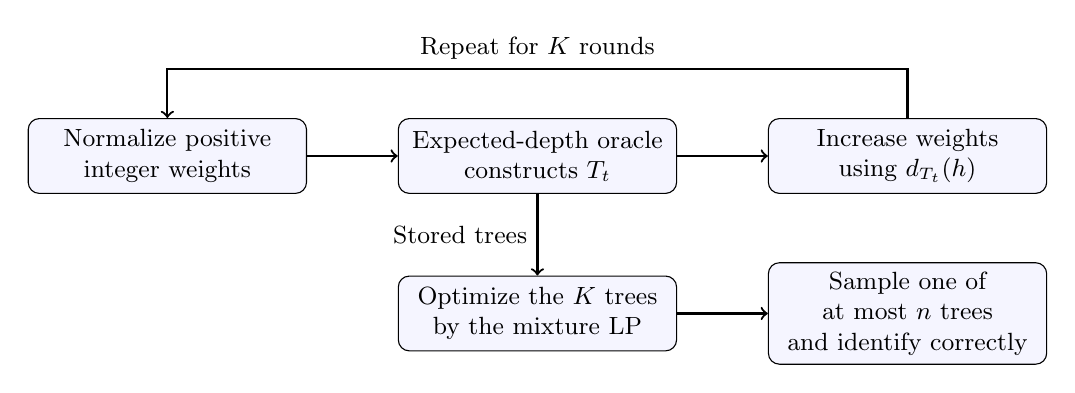
\begin{tikzpicture}[
  box/.style={draw,rounded corners,fill=blue!4,align=center,
              text width=3.3cm,minimum height=0.95cm,font=\small},
  arrow/.style={->,thick},
  every node/.style={font=\small}]
\node[box] (prior) at (0,0) {Normalize positive\\integer weights};
\node[box] (oracle) at (4.7,0) {Expected-depth oracle\\constructs $T_t$};
\node[box] (update) at (9.4,0) {Increase weights\\using $d_{T_t}(h)$};
\node[box] (master) at (4.7,-2) {Optimize the $K$ trees\\by the mixture LP};
\node[box] (sample) at (9.4,-2) {Sample one of at most $n$ trees\\and identify correctly};
\draw[arrow] (prior)--(oracle);
\draw[arrow] (oracle)--(update);
\draw[arrow] (update.north)--(9.4,1.1)--node[above]
  {Repeat for $K$ rounds}(0,1.1)--(prior.north);
\draw[arrow] (oracle)--node[left]{Stored trees}(master);
\draw[arrow] (master)--(sample);
\end{tikzpicture}
\caption{Preprocessing uses the oracle to build trees and the master LP
to choose their probabilities. Each later identification run samples
one complete tree and follows it. Weight updates and the LP run during
preprocessing, before the hidden hypothesis is queried.}
\label{fig:randomized-flow}
\end{figure}

To compare this construction with the best possible randomized
strategy, we first identify its benchmark. The hardest prior is the
dual of the tree-mixture problem: even an ideal mixture must pay
the optimal expected cost of that prior. Since the dual benchmark is
an expected-depth optimum for some prior, an expected-depth
approximation oracle can bound its value in every round.
\begin{proposition}[The comparison game and its entropy lower bound]
\label{prop:randomized-duality}
The optimum in \eqref{eq:randomized-objective} also covers adaptive
zero-error randomized algorithms that terminate almost surely on
every hypothesis. It satisfies
\begin{equation}\label{eq:randomized-duality}
 R^*=\max_{\pi\in\Delta(\HH)}\OPT_E(\pi)
       \ge\log_2n.
\end{equation}
The dual maximum ranges over the full simplex and may assign zero
mass; Algorithm~\ref{alg:randomized-mixture} supplies strictly positive
priors to the expected-depth oracle.
\end{proposition}

The benchmark bounds the oracle's cost on every round's prior.
The regret proposition turns these changing weighted averages into a
bound for \emph{each} hypothesis: a repeatedly slow hypothesis gains
influence until the oracle's weighted cost reflects its depth. The
resulting average-depth bound is for the uniform distribution over
generated trees. Since the restricted master LP also considers this
mixture, its optimized maximum per-hypothesis cost is no greater.
\begin{proposition}[Depth-scaled multiplicative weights]
\label{prop:randomized-regret}
For any sequence of proper oracle trees, let $\pi_t$ be the normalized
weights before round $t$. The uniform mixture of the generated trees
satisfies
\begin{equation}\label{eq:randomized-regret}
 R(\mu^{\rm unif})\le
    (1+\eta)\frac1K\sum_{t=1}^K c_{\pi_t}(T_t)
    +\frac{2L\ln n}{\eta K}.
\end{equation}
\end{proposition}

The uniform mixture in the regret bound may contain many trees.
The master LP keeps its guarantee while producing a concise
strategy. The next proposition also ensures that the repeated
priors and the final random choice can be implemented exactly.
\begin{proposition}[Exact rational construction and sparse optimal mixing]
\label{prop:randomized-compression}
Every iterative prior is strictly positive and rational, with encoding
length polynomial in $n,K$ and the encoding length of $\eta$.
The LP \eqref{eq:randomized-master-lp} is polynomial in size and has an
optimal basic solution supported on at most $n$ trees. Its value is
at most $R(\mu^{\rm unif})$. Its probabilities have polynomial encoding
length and admit exact sampling with an expected polynomial number
of fair random bits. Every sampled query run is correct and uses at
most $n-1$ supplied tests.
\end{proposition}

\begin{proofstrategy}
\begin{enumerate}
\item View hypotheses and legal trees as the two sides of a finite
      game. Its hardest prior lower-bounds every randomized strategy.
\item Increase the weight of hypotheses with large current depths.
      The potential comparison bounds each hypothesis's average
      depth by the oracle's average weighted cost.
\item Optimize the generated mixture by a small LP. The entropy
      lower bound makes the regret term a multiplicative tolerance;
      a basic solution leaves at most $n$ trees to sample.
\end{enumerate}
\end{proofstrategy}

Together, these statements transfer the oracle's approximation
coefficient to the new objective, with a controllable tolerance.
The extra work constructs and mixes trees; the query procedures
inside each tree remain those of the expected-depth oracle.
\begin{theorem}[Transfer to randomized per-hypothesis depth]
\label{thm:randomized-transfer}
For every rational $0<\varepsilon\le1$, Algorithm~\ref{alg:randomized-mixture},
with the calibration at the end of this section, satisfies
\[
 R(\mu)<(\alpha+\varepsilon)R^*\qquad(n\ge2).
\]
It makes $O(n/\varepsilon^2)$ calls to the expected-depth oracle,
uses only positive rational priors, and returns a mixture of at most
$n$ legal trees. If the oracle is polynomial-time in its rational
input, preprocessing is polynomial in the input size and
$1/\varepsilon$. For a singleton, return its leaf with zero queries.
\end{theorem}
\begin{proof}
Proposition~\ref{prop:randomized-duality} and \eqref{eq:randomized-oracle} give
$c_{\pi_t}(T_t)\le\alpha R^*$ in every round. Apply
Proposition~\ref{prop:randomized-regret} and use
$\ln n\le(\ln2)R^*<R^*$ to obtain
\[
 R(\mu^{\rm unif})<
 \left[(1+\eta)\alpha+\frac{2L}{\eta K}\right]R^*.
\]
The final calibration makes the bracket at most
$\alpha+\varepsilon$. Proposition~\ref{prop:randomized-compression} transfers this
bound to the optimized mixture and supplies positivity, legality,
and bit complexity. The chosen $K$ gives the stated number of calls.
\end{proof}

\subsection{Proofs of the supporting propositions}

\subsubsection{The hardest prior is the dual comparison object}

The game interpretation rests on two facts. First, fixing the random
seed turns the policy into a proper tree, and contracting constant
queries can only shorten its paths. Averaging over seeds therefore
gives a tree mixture whose expected depth on each hypothesis is at most
the algorithm's. Second, the mixture optimum equals the expected-depth
cost of its hardest prior. We prove these in order, then use the resulting
lower bound to absorb the weight-update error.

\begin{claim}[Random seeds reduce to a finite proper-tree mixture]
\label{clm:randomized-seed-mixture}
Any zero-error randomized algorithm terminating almost surely on each
hypothesis induces a mixture over $\mathcal T$ whose expected depth on
each hypothesis is at most that of the algorithm.
\end{claim}
\begin{proof}
Condition on a complete random seed. Since $\HH$ is finite, outside
a probability-zero union of events the resulting deterministic
policy terminates correctly on every hypothesis. The union of its
$n$ finite paths is a finite identification tree. Delete unreachable
branches and contract queries constant on their current states.
Every retained query splits a state properly, so the resulting tree
has $n$ leaves, $n-1$ internal nodes, and maximum depth at most $L$.
The finite supplied query family admits only finitely many such
labeled trees. Pushing the seed distribution onto these trees gives
the required mixture. Conversely, sampling any such mixture gives
a legal zero-error strategy.
\end{proof}

After fixing the seed, every strategy is a proper legal tree. The
finite family of these trees defines a mixture LP for the analysis;
its dual assigns mass to hypotheses, giving precisely the prior needed
by the expected-depth oracle. The algorithm constructs a polynomial-size
subset of this finite family, then optimizes the mixture over those trees.
\begin{claim}[Finite LP duality identifies the hardest prior]
\label{clm:randomized-finite-dual}
The finite-tree mixture optimum equals
$\max_{\pi\in\Delta(\HH)}\min_{T\in\mathcal T}c_\pi(T)$.
\end{claim}
\begin{proofstrategy}
We derive the dual by assigning one multiplier to each hypothesis
constraint and one to mixture normalization. The Lagrangian gives the
dual constraints directly; weak duality is then explicit, and finite
LP strong duality completes the equality.
\end{proofstrategy}
\begin{proof}
Write the full mixture LP with one variable $\mu_T$ for each
$T\in\mathcal T$, the depth inequalities, and normalization
$\sum_T\mu_T=1$. Its dual is
\[
 \begin{aligned}
  \text{maximize}\quad&\lambda,\\
  \text{subject to}\quad&
       \lambda\le\sum_h\pi_hd_T(h) &&(T\in\mathcal T),\\
   &\pi_h\ge0,\qquad\sum_h\pi_h=1.
 \end{aligned}
\]
Here one may leave the primal variable $r$ unrestricted: for
$n\ge2$, every depth is at least one, so its inequalities already
force $r\ge1$. To derive the dual, assign nonnegative multipliers
$\pi_h$ to $\sum_T\mu_Td_T(h)-r\le0$ and a free multiplier
$\lambda$ to $1-\sum_T\mu_T=0$. The Lagrangian is
\[
\begin{aligned}
 \mathcal L(r,\mu;\pi,\lambda)
 &=r+\sum_h\pi_h\left(\sum_T\mu_Td_T(h)-r\right)
                      +\lambda\left(1-\sum_T\mu_T\right)\\
 &=r\left(1-\sum_h\pi_h\right)+\lambda
                  +\sum_T\mu_T\bigl(c_\pi(T)-\lambda\bigr).
\end{aligned}
\]
Its infimum over free $r$ and nonnegative $\mu_T$ is finite exactly
when $\sum_h\pi_h=1$ and $c_\pi(T)\ge\lambda$ for every $T$.
Under those conditions the infimum is $\lambda$, giving the stated
dual. In particular, weak duality is visible directly:
\[
 \lambda\le\sum_T\mu_Tc_\pi(T)
       =\sum_h\pi_h\sum_T\mu_Td_T(h)
       \le\sum_h\pi_hr=r.
\]
The first inequality averages the dual constraint over a normalized
mixture. The equality exchanges two finite sums, and the last
inequality weights the primal depth constraints by the nonnegative
$\pi_h$. Their sum is one, which gives the final equality.
The finite primal is feasible and bounded: any proper tree gives
a feasible pure mixture with $1\le r\le L$. Thus
finite LP duality gives equality of its optimum and this dual
optimum. For fixed $\pi$, the largest feasible $\lambda$ is exactly
$\min_Tc_\pi(T)$. The dual permits zero-mass hypotheses because it
defines the comparison benchmark. The algorithm itself uses strictly
positive priors, as required by the oracle.
\end{proof}

The dual identity already gives the comparison benchmark. We also
need its scale: identifying $n$ possibilities requires logarithmic
expected depth under the uniform prior. This ensures that the
additive regret term becomes a multiplicative tolerance.
\begin{claim}[The uniform prior provides a logarithmic lower bound]
\label{clm:randomized-uniform-lower}
Every identifying binary tree has uniform-prior expected depth at
least $\log_2n$.
\end{claim}
\begin{proof}
Its leaf depths satisfy Theorem~\ref{thm:kraft}. By convexity of
$2^{-x}$,
\[
 2^{-\frac1n\sum_hd_T(h)}
   \le\frac1n\sum_h2^{-d_T(h)}\le\frac1n.
\]
The first inequality is Jensen's inequality and the second is Kraft's
bound divided by $n$. Taking $-\log_2$ reverses both inequalities
and gives the claim. Applying Claim~\ref{clm:randomized-finite-dual} to
the uniform prior proves \eqref{eq:randomized-duality}.
\end{proof}

\subsubsection{A weight potential bounds every hypothesis's depth}

Consider a hypothesis that remains slow in many generated trees.
Its weight must grow quickly. The sum of all weights, however,
grows according to the oracle's cost on the current prior. Comparing
these two growth rates bounds every hypothesis's average depth by
the oracle's average weighted cost. Scaling depths by $L$ lets the
same calculation apply to every proper tree.

\begin{claim}[Individual weight growth is paid by total weight growth]
\label{clm:randomized-weight-growth}
For the scaled multiplicative-weights update in
\eqref{eq:randomized-integer-update} and
$g_{h,t}=d_{T_t}(h)/L\in[0,1]$,
\[
 \ln(1+\eta)\sum_{t=1}^Kg_{h,t}
 \le\ln n+\eta\sum_{t=1}^K\sum_g\pi_{g,t}g_{g,t}
 \quad\text{for every }h.
\]
\end{claim}
\begin{proofstrategy}
Remove the common integer factor so the normalized priors are
unchanged. A single hypothesis's weight grows at a rate set by its
depth, while the sum of all weights grows at a rate set by the current
prior's mean depth. Comparing these bounds gives the claim.
\end{proofstrategy}
\begin{proof}
Write $\widehat w_{h,t}=w_{h,t}/(qL)^{t-1}$ for the integer weights
with their common factor removed. This leaves their normalized
prior unchanged and makes their update $1+\eta g_{h,t}$.
Concavity of $x\mapsto\ln(1+\eta x)$ places its graph above the
chord between $x=0$ and $x=1$, giving
$\ln(1+\eta x)\ge x\ln(1+\eta)$, so each final weight obeys
\[
 \ln\widehat w_{h,K+1}\ge\ln(1+\eta)\sum_tg_{h,t}.
\]
For their sum $\widehat W_t$, initially $\widehat W_1=n$ and
\[
 \frac{\widehat W_{t+1}}{\widehat W_t}
    =1+\eta\sum_h\pi_{h,t}g_{h,t}.
\]
Taking logarithms and summing the successive total-weight ratios gives
\[
\begin{aligned}
 \ln\widehat W_{K+1}
 &=\ln n+\sum_{t=1}^K
          \ln\left(1+\eta\sum_g\pi_{g,t}g_{g,t}\right)\\
 &\le\ln n+\eta\sum_{t=1}^K\sum_g\pi_{g,t}g_{g,t}.
\end{aligned}
\]
The inequality uses $\ln(1+x)\le x$ with nonnegative $x$.
For each $h$, positivity and
$\widehat w_{h,K+1}\le\widehat W_{K+1}$ imply
\[
 \ln(1+\eta)\sum_tg_{h,t}
 \le\ln\widehat w_{h,K+1}
 \le\ln\widehat W_{K+1},
\]
which is the required comparison.
\end{proof}

The growth comparison is expressed in normalized depths and
logarithms. For the uniform mixture,
$R(\mu^{\rm unif})=\max_h K^{-1}\sum_t d_{T_t}(h)$; thus rescaling
the claim by $L/K$ converts its per-hypothesis sums to the objective
in \eqref{eq:randomized-objective}. Bounding the two logarithmic
coefficients then gives the explicit regret bound.
\begin{claim}[The potential comparison gives the stated regret]
\label{clm:randomized-regret-rescaling}
Claim~\ref{clm:randomized-weight-growth} implies \eqref{eq:randomized-regret}.
\end{claim}
\begin{proof}
Multiply the bound in Claim~\ref{clm:randomized-weight-growth} by
$L/[K\ln(1+\eta)]$ and maximize over $h$. Since
$\sum_g\pi_{g,t}g_{g,t}=c_{\pi_t}(T_t)/L$, the weighted-depth
term becomes the average oracle cost, and we obtain
\[
 R(\mu^{\rm unif})\le
 \frac{\eta}{\ln(1+\eta)}\frac1K\sum_tc_{\pi_t}(T_t)
 +\frac{L\ln n}{K\ln(1+\eta)}.
\]
The integral for $\ln(1+\eta)$ gives
\[
 \ln(1+\eta)=\int_0^\eta\frac{dx}{1+x}
       \ge\frac{\eta}{1+\eta}\ge\frac{\eta}{2}
       \qquad(0<\eta\le1).
\]
The first inequality bounds the integrand below by its endpoint
value $1/(1+\eta)$; the second uses $1+\eta\le2$.
Therefore
$\eta/\ln(1+\eta)\le1+\eta$ and
$1/\ln(1+\eta)\le2/\eta$. Substituting separately into the
nonnegative mean-cost and error terms gives
\[
 R(\mu^{\rm unif})\le
 (1+\eta)\frac1K\sum_tc_{\pi_t}(T_t)
                  +\frac{2L\ln n}{\eta K},
\]
as claimed.
\end{proof}

\subsubsection{Integer updates and a basic LP solution give a finite strategy}

We analyze the updates with logarithmic potentials and implement them
using positive integer weights; normalization gives the exact rational
priors supplied to the oracle. A basic solution of the master LP bounds
the number of stored trees and the bit length of their probabilities.
Exact sampling then completes the construction and preserves the query
guarantee.

\begin{claim}[All oracle inputs have strictly positive rational weights]
The updates \eqref{eq:randomized-integer-update} preserve positivity
and have polynomial encoding length.
\end{claim}
\begin{proof}
The initial weights are one. Every update factor is a positive
integer at most $(p+q)L$. After $K$ rounds, each weight therefore
has $O(K\log((p+q)L)+1)$ bits. Normalization adds at most
$\lceil\log_2n\rceil$ bits to the denominator. All priors are
strictly positive, so every call meets the oracle's hypothesis.
The generated proper trees have $O(nK)$ total nodes; their depth
matrix consists of integers at most $L$.
\end{proof}

All generated trees can therefore be stored in a polynomial-size
depth matrix. The LP has one column per generated tree and $n$
hypothesis-depth constraints; these constraints determine the worst
expected depth. An optimal basic solution uses this structure to
retain a small support.
\begin{claim}[An optimal basic mixture uses at most $n$ trees]
\label{clm:randomized-basic-support}
The LP \eqref{eq:randomized-master-lp} has an optimal basic solution
with at most $n$ positive tree probabilities and polynomial-bit
rational coefficients.
\end{claim}
\begin{proofstrategy}
Put the LP in standard form and use positivity of the objective
variable to bound the number of tree probabilities in a basic
solution. Then bound the basis determinants to control the bit length
of those probabilities.
\end{proofstrategy}
\begin{proof}
Its uniform mixture is feasible. Replacing every depth inequality
by
\[
 \sum_t\mu_td_{T_t}(h)+s_h-r=0,\qquad s_h\ge0,
\]
gives standard form with $n+1$ equalities and nonnegative variables
$\mu_t,s_h,r$. Because $n\ge2$, every proper tree has depth at least
one on every hypothesis. Since the probabilities sum to one, each
depth inequality therefore forces $r\ge1$, so the variable $r$ is
positive in every feasible solution. A basic solution has at most
$n+1$ positive variables, leaving at most
$n$ for tree probabilities. If some equalities are dependent, the basis
dimension decreases and the same support bound remains valid. A finite
optimal basic solution exists, and its
integer basis matrix has entries of absolute value at most $L$.
For completeness, let $b\le n+1$ be the basis size. The basis
matrix $B$ is nonsingular and integer, so $|\det B|\ge1$.
Each of its columns has Euclidean norm at most $\sqrt b\,L$.
Hadamard's bound and Cramer's rule therefore give
\[
 1\le|\det B|\le(\sqrt b\,L)^b,\qquad
 |\det B_i|\le(\sqrt b\,L)^b,\qquad
 x_i=\frac{\det B_i}{\det B}.
\]
The bound on $B_i$ also holds because the right-hand side has
entries zero or one, and $L\ge1$. Each numerator and denominator
thus needs $O(b(\log b+\log L)+1)$ bits. In particular the tree
probabilities have polynomial encoding length. Rational LP algorithms,
followed by exact basis extraction on the optimal face, find such
an optimal basic solution in polynomial time
\cite{khachiyan1979}. The uniform mixture is feasible, so the optimized
value is at most $R(\mu^{\rm unif})$.
\end{proof}

The sparse LP solution assigns probabilities to the retained trees.
Each run samples one tree and executes it from root to leaf. Its
rational probabilities allow an exact draw using fair bits, so the
execution preserves the zero-error query guarantee.
\begin{claim}[The compressed mixture is exactly sampleable]
\label{clm:randomized-exact-sampling}
The optimized rational mixture gives a legal zero-error execution
with at most $L$ queries and expected polynomial sampling cost.
\end{claim}
\begin{proofstrategy}
Clear the rational probabilities to obtain integer interval lengths.
Rejection sampling produces a uniform integer in their common range,
which selects a tree with exactly its LP probability and finite
expected bit cost.
\end{proofstrategy}
\begin{proof}
By Claim~\ref{clm:randomized-basic-support}, take a common denominator
$D$ for its at most $n$ polynomial-bit probabilities;
its encoding length is polynomial. Explicitly, if their denominators
are $b_1,\ldots,b_s$, take $D=\prod_{i=1}^s b_i$; then
$\log_2D=\sum_i\log_2b_i$ is polynomial. Writing the probabilities
as $a_i/D$ gives nonnegative integer interval lengths with
$\sum_i a_i=D$. Draw a uniform integer from
$\{0,\ldots,D-1\}$ by fair bits and rejection, then use the
cumulative integer probability intervals. Rejection makes every
accepted integer equiprobable, so an interval of length $a_i$ has
probability $a_i/D$. If $D=1$, select the sole supported tree
deterministically. Otherwise each attempt uses
$\lceil\log_2D\rceil$ bits and is accepted with probability
greater than $1/2$, so the expected number of attempts is less
than two: with $b=\lceil\log_2D\rceil$, each $b$-bit draw is uniform
on $\{0,\ldots,2^b-1\}$, and
$D/2^b>1/2$. Conditioning on a draw below $D$ makes it uniform
on the desired range.
The sampled tree identifies every hypothesis and has
depth at most $L$. This completes the compression proposition.
\end{proof}

The two optimization viewpoints also give a useful stopping
certificate. The restricted master LP supplies an upper bound on
$R^*$ because its mixture is a feasible strategy, while
\[
 \max_t\frac{c_{\pi_t}(T_t)}\alpha\le R^*
\]
supplies a lower bound by \eqref{eq:randomized-oracle} and
\eqref{eq:randomized-duality}. Their ratio is an instance-specific
certificate. Stop early when it meets the desired factor; otherwise,
the fixed-round guarantee still applies.

\subsection{Calibration and the strongest resulting guarantees}

The preceding proof separates the oracle's approximation loss from
the loss due to finitely many weight-update rounds. Split the desired
tolerance equally between these two terms; the following choices
make that split explicit.

\begin{parameterchoice}
For a fixed rational oracle coefficient $\alpha\ge1$ and target
$0<\varepsilon\le1$, choose
\begin{equation}\label{eq:randomized-calibration}
 \eta=\frac{\varepsilon}{2\alpha},\qquad
 K=\left\lceil\frac{8\alpha(n-1)}{\varepsilon^2}\right\rceil.
\end{equation}
The definition of $\eta$ gives $\alpha\eta=\varepsilon/2$. For the
second term, use $L=n-1$ and the lower bound on the ceiling-defined $K$:
\[
 \frac{2L}{\eta K}
 \le \frac{2L}{(\varepsilon/(2\alpha))(8\alpha L/\varepsilon^2)}
 =\frac{\varepsilon}{2}.
\]
Thus each error term is at most $\varepsilon/2$, and their sum is at
most $\varepsilon$.
\end{parameterchoice}

The oracle and duality give
$c_{\pi_t}(T_t)\le\alpha\OPT_E(\pi_t)\le\alpha R^*$ in each round.
Substitution into the regret inequality yields
\[
\begin{aligned}
 R(\mu^{\rm unif})
 &\byref{Prop.}{prop:randomized-regret}{\le}
 (1+\eta)\alpha R^*+\frac{2L\ln n}{\eta K}\\
 &\byref{Eq.}{eq:randomized-calibration}{\le}
 \left(\alpha+\frac{\varepsilon}{2}\right)R^*
                      +\frac{\varepsilon}{2}\ln n\\
 &\byref{Prop.}{prop:randomized-duality}{<}(\alpha+\varepsilon)R^*.
\end{aligned}
\]
The final inequality is strict because $n\ge2$ and
$\ln n=(\ln2)\log_2n<\log_2n\le R^*$.
The optimized mixture has cost at most that of the uniform one.

The current expected-depth certificate in
Section~\ref{sec:two-phase} gives the rational valid oracle
coefficient $\alpha=5.18297551$. Choosing
$\varepsilon=1/4000000$ in the single mixture algorithm yields
\[
 R(\mu)<5.18297576\,R^*<5.182976\,R^*.
\]
This is the best polynomial factor established here for the
randomized per-hypothesis objective. The small tolerance makes the
iteration constant large; the parameterized theorem and the
optimized master LP allow more practical tolerance choices.

Using a stronger expected-depth oracle preserves the prior updates and
mixture LP while improving the guarantee for this randomized objective.
The quasipolynomial oracle gives the stronger factor, and its running
time carries over to preprocessing.
\begin{corollary}[Quasipolynomial randomized per-hypothesis approximation]
\label{cor:randomized-quasipolynomial}
For every fixed rational $\varepsilon>0$, the same LP-compressed
mixture algorithm has a supplied-query quasipolynomial
$(2+\varepsilon)$ approximation for $R^*$. For
$0<\varepsilon\le1$, its time is
$(mn)^{O(\varepsilon^{-1}\log n)}$ times a polynomial in input
bit length, and its mixture is supported on at most $n$ trees.
\end{corollary}
\begin{proof}
Use the expected-depth oracle of
Theorem~\ref{thm:qp-two-plus-epsilon} with coefficient
$\alpha=2+\varepsilon/2$, and apply the transfer theorem with
tolerance $\varepsilon/2$. The factor is strictly below
$2+\varepsilon$ for $n\ge2$. There are
$\lceil32\alpha(n-1)/\varepsilon^2\rceil$ oracle calls, whose
positive rational priors have polynomial encoding length. These
calls and the master LP preserve the oracle's stated
quasipolynomial running-time form. For $\varepsilon>1$, use
$\varepsilon=1$; a singleton again returns its leaf.
\end{proof}
